\documentclass[a4paper, top=10mm]{article}
%for writing from the top
\usepackage{fullpage}
%for math
\usepackage{amsmath}
\usepackage{mathrsfs}
\usepackage{amsthm}
%for images
\usepackage{graphicx}
%for color
\usepackage{xcolor}
%for title
\title{\textbf{\huge{Treasure Safe}}}
\author{Enigma n\textsuperscript{o}8}
\date{25\textsuperscript{th} June 2024}

\newtheorem*{hint}{Hint}

\addtolength{\voffset}{-2cm}
\addtolength{\textheight}{5cm}


\begin{document}
	\maketitle
	
	\Large
	The safe code is made of 4 digits, all different.
	
	Four people have tired before you, and the master keeping the safe gave some clues:
	\begin{itemize}
		\item 8 0 7 4: Two numbers are correct and well placed.
		\item 3 7 8 2: A number is misplaced but correct.
		\item 7 5 1 9: Nothing is correct.
		\item 5 1 2 0: Two digits are misplaced but correct.
	\end{itemize}
	
	What is the safe code?
	
	\vspace{2cm}
	
	\begin{center}
		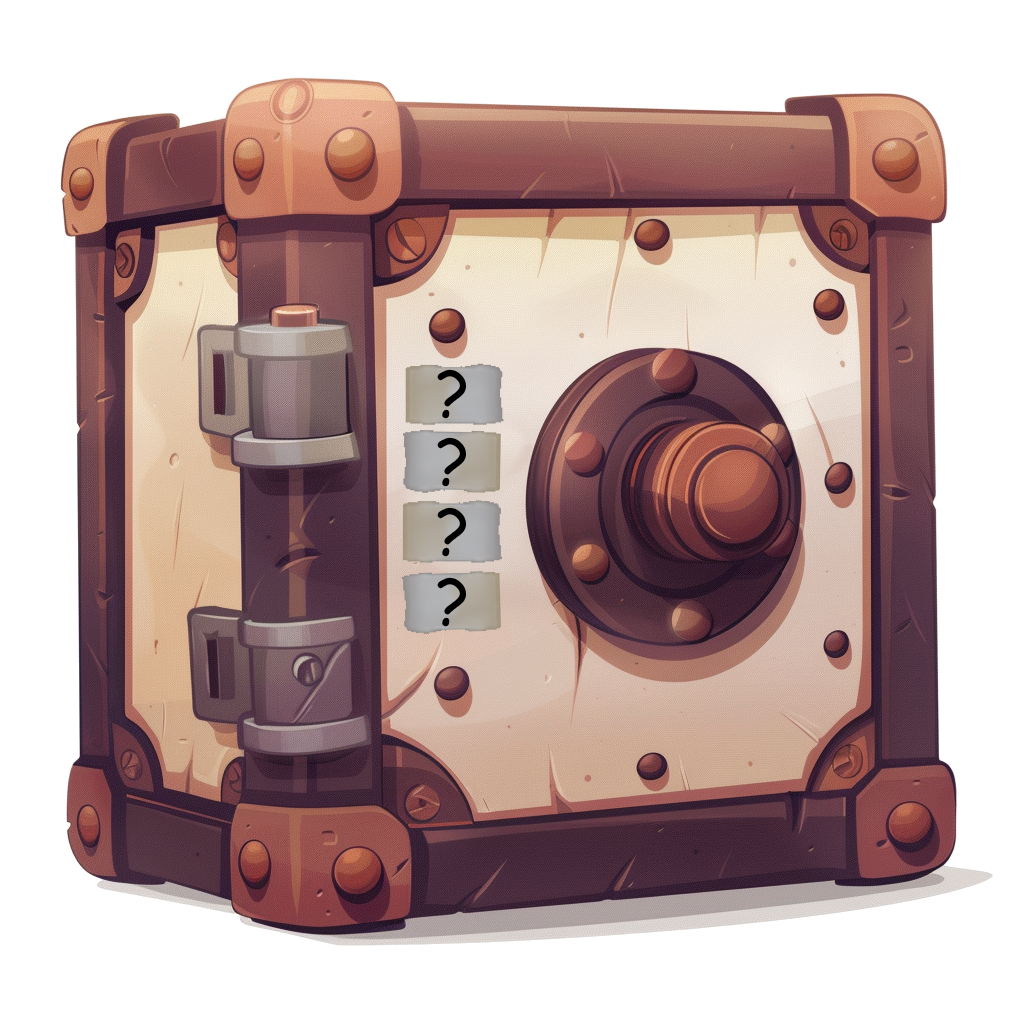
\includegraphics[width=\linewidth]{08safe.png}
	\end{center}
	

	
	
\end{document}